\documentclass{standalone}
\usepackage{tikz}

\usetikzlibrary{calc}

\begin{document}

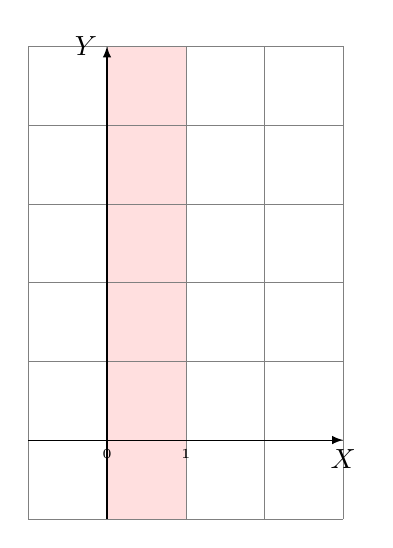
\begin{tikzpicture}
  \path[fill=red!50,opacity=.25] (0,-1) rectangle (1,5);
  \draw[ultra thin,gray] (-1,-1) grid (3,5);
  \draw[-latex] (-1,0) -- (3,0) node[below] {$X$};
  \draw[-latex] (0,-1) -- (0,5) node[left] {$Y$};
  \node[below,font=\tiny] at (0,0) {0};
  \node[below,font=\tiny] at (1,0) {1};
\end{tikzpicture}

\end{document}